\section{实验验证}

本章介绍实验部分。第一节为实验平台软硬件配置。第二节介绍LLM模型与数据集选取,以及实验参数设置。第三节针对基于开销感知的内存优化策略,进行吞吐率测试。第四节针对基于公平性的用户请求调度策略,进行实时性测试。第五节分析张量交换与张量重算预测误差。第六节进行其它测试工作。

\subsection{实验环境}

本文开展实验使用的服务器软硬件配置如表\ref{Table:实验平台的软硬件配置}所示。使用Intel(R) Xeon(R) CPU和NVIDIA A800 80GB GPU作为硬件环境,使用CUDA-11.8、PyTorch-2.0.l、Ray2.7.1以及vLLM-0.2.5作为底层框架进行开发。服务器使用PCIe连接实现GPU-CPU通信。

\begin{table}[H]
  \centering
  \caption{实验平台的软硬件配置}
  \label{Table:实验平台的软硬件配置}
  \renewcommand{\arraystretch}{1.25}
  \small
  \begin{tabular}{c c}
    \toprule
    \textbf{软件/硬件} & \textbf{型号/版本} \\ 
    \midrule
    CPU & Intel(R) Xeon(R) CPU @ 2.60GHz  \\ 
    GPU & NVIDIA A800 PCIE 80GB \\ 
    OS & CentOS Linux 7 (Core) \\ 
    CUDA & 11.8 \\ 
    PyTorch & 2.0.1 \\ 
    Ray & 2.7.1 \\
    vLLM & 0.2.5 \\ 
    \bottomrule
  \end{tabular}
\end{table}

% 服务器使用PCIe连接实现GPU-CPU通信。PCIe传输带宽在传输数据量不同时差异显著,表\ref{Table:PCIe双向传输带宽}列出了部分情况。在计算张量交换开销时,需要根据单次实际传输的数据量(一般是一个Block或其中的一部分)找到对应的传输带宽值。

% \begin{table}[H]
%   \centering
%   \caption{PCIe双向传输带宽}
%   \label{Table:PCIe双向传输带宽}
%   \renewcommand{\arraystretch}{1.2}
%   \small
%   \begin{tabular}{c c c}
%     \toprule
%     \textbf{传输量(B)} & \textbf{HtoD(MB/s)} & \textbf{DtoH(MB/s)} \\
%     \midrule
%     1024 & 0.19 & 0.24 \\ 
%     2048 & 0.60 & 0.72 \\ 
%     4096 & 1.20 & 1.49 \\ 
%     8192 & 1.07 & 2.97 \\ 
%     16384 & 4.16 & 5.79 \\ 
%     32768 & 7.76 & 9.35 \\ 
%     102400 & 14.27 & 16.49 \\ 
%     204800 & 18.30 & 20.24 \\ 
%     409600 & 21.17 & 22.57 \\ 
%     \bottomrule
%   \end{tabular}
% \end{table}

\begin{figure*}[!htbp]
  \centering
  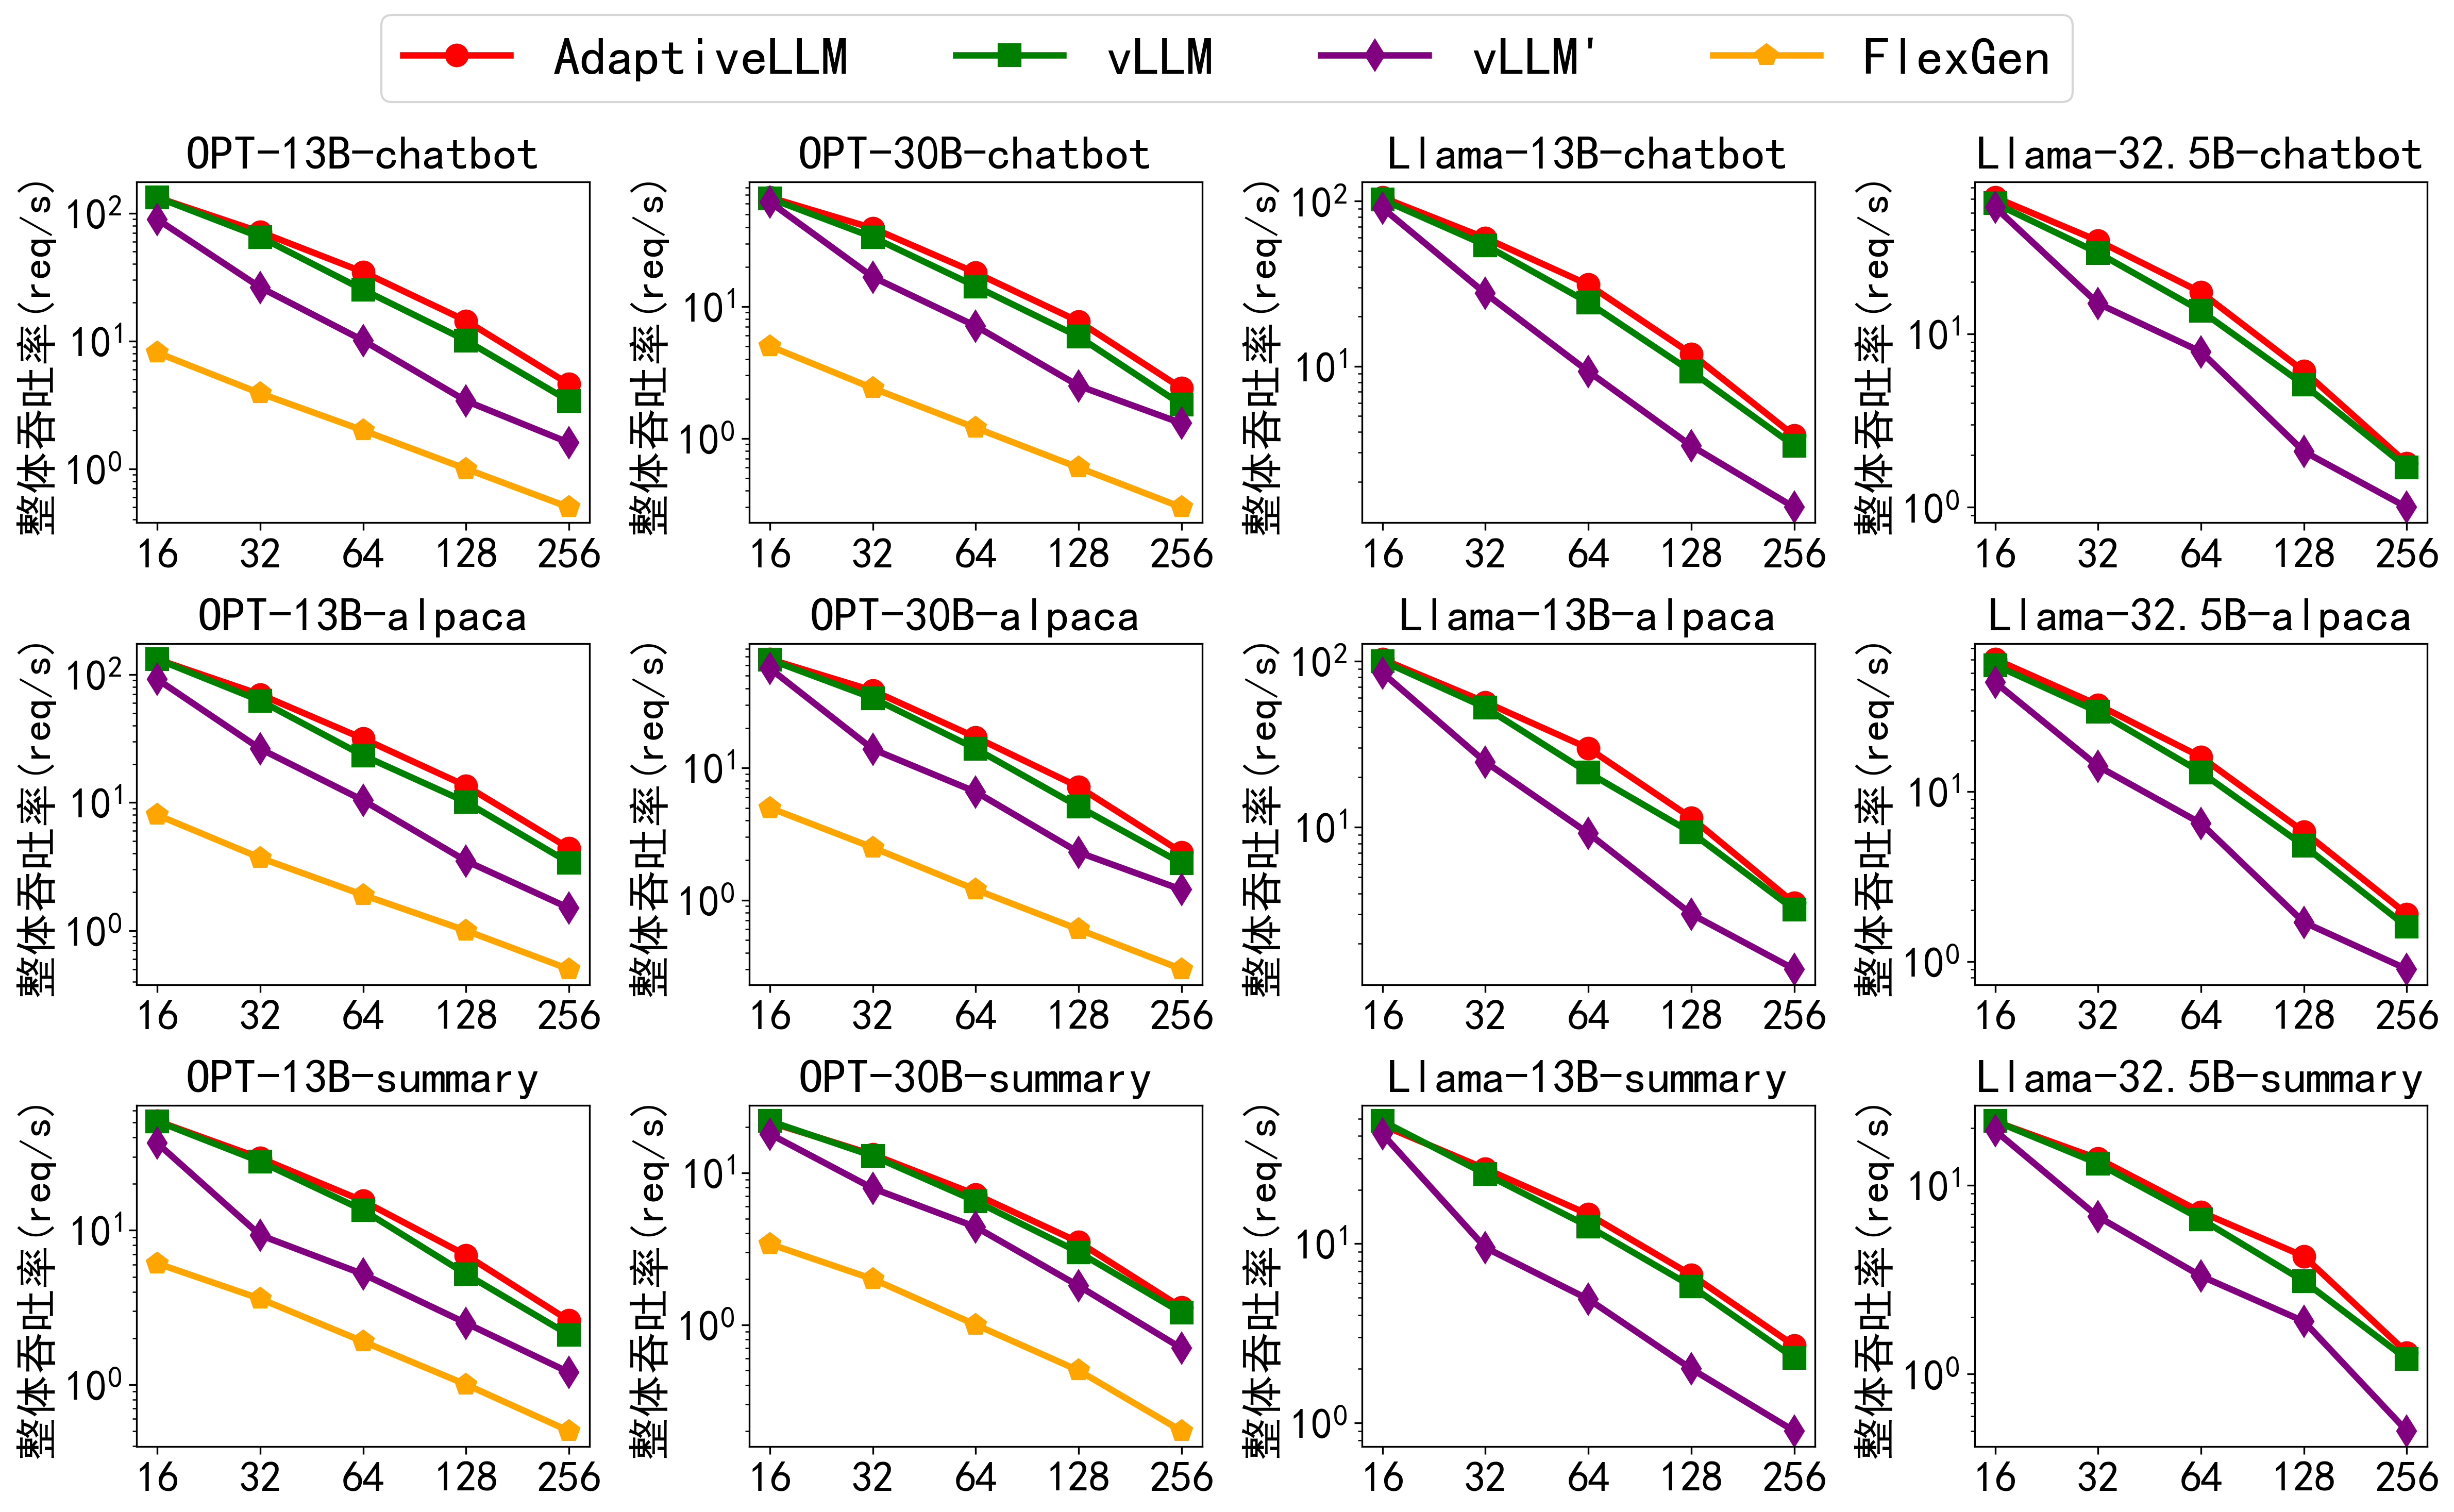
\includegraphics[width=0.9\linewidth]{推理任务吞吐率.png}
  \caption{推理任务吞吐率}
  \label{Fig:推理任务吞吐率}
\end{figure*}

\subsection{模型与数据集}

本文选用OPT~\cite{OPT}(OPT-13B、OPT-30B)和Llama~\cite{Llama}(Llama-13B、Llama-32.5B)作为实验模型,在三个常见数据集(Chatbot~\cite{Chatbot}、Alpaca~\cite{Alpaca}、Summary~\cite{Summary})上进行测试。数据集信息如表\ref{Table:实验数据集选取}所示。

\begin{table}[H]
  \centering
  \caption{实验数据集选取}
  \label{Table:实验数据集选取}
  \renewcommand{\arraystretch}{1.25}
  \small
  \begin{tabular}{c c c c}
    \toprule
    \textbf{数据集} & \textbf{样本总数} & \textbf{平均输入长度} & \textbf{任务类型} \\
    \midrule
    Chatbot & 258064 & 17.02 & 对话类 \\
    Alpaca & 68912 & 19.66 & 指令类 \\
    Summary & 1799 & 340.48 & 摘要类 \\
    \bottomrule
  \end{tabular}
\end{table}

Chatbot和Alpaca中大多数序列长度较短,而Summary中序列长度展现出很大差异性,且包含长序列。它们涵盖了LLM应用程序面临的大部分场景。

实验过程中的参数设置模拟LLM应用程序在多任务并发场景下的运行状态。{\color{red}可用GPU内存越多,调度器支持的批处理大小就越大,因此推理任务的吞吐率较高。本文将GPU Block数量设置为128,模拟GPU内存不足时的用户请求抢占场景。同时,可用CPU内存较多时,内存优化决策器偏向于使用张量交换来释放内存。本文将CPU Block数量设置为64,使得内存优化决策器在CPU内存不足时调用张量重算,而非简答地将被抢占用户请求交付张量交换执行器。}针对12个实验组,在相应数据集中使用简单随机抽样法选取1000个样本进行后续测试。

%wsq 实验部分改一下顺序,重要的实验放前面。吞吐率测试,实时性测试,执行时间预测,开销分析。

% wsq 这应该算是motivation实验,基于这个观察你才有空间去选择策略。不应该出现在大实验中。
% \subsection{重算与交换的开销对比}

% 本文对OPT-13B、OPT-30B、Llama-13B和Llama-32.5B进行开销对比测试,其结果如图\ref{Fig:交换与重算开销对比}所示。当序列长度较小时,交换开销小于重算开销;随着序列长度的增加,二者大小关系反转。原因如下:  \par

% 自注意力机制内核采用并行计算策略,每个线程只计算一个token的qkv张量及注意力值。随着token数量增多,并行执行的线程数量增加,线程间同步开销随之上升,而单线程计算量不变。因此张量重算开销随序列长度增加呈亚线性增长。而由公式\ref{Eq:Swap Overhead}、\ref{Eq:Block Mem}、\ref{Eq:KV Cache Mem}可知,张量交换开销与序列长度呈近似正比关系。因此,张量重算开销的增长速度小于张量交换开销。  \par

% \begin{figure}[!htbp]
%   \centering
%   \includegraphics[width=0.9\linewidth]
%   {交换与重算开销对比.png}
%   \caption{交换与重算开销对比}
%   \label{Fig:交换与重算开销对比}
% \end{figure}

% 在贪心采样策略下,对于长序列(如Summary数据集中的部分样本),无论是vLLM还是AdaptiveLLM,都偏向于使用重算,两种策略带来的抢占行为没有差异。对于短序列(如Chatbot和Alpaca数据集),vLLM使用重算,而AdaptiveLLM使用开销较小的交换,此时能够带来吞吐率提升。在LLM实际应用场景中,大多数序列的长度较短,使得张量交换在提升性能上拥有明显优势。而当长序列较多,或者CPU内存空间不足时,张量重算技术能够发挥优势。 

\subsection{吞吐率测试}

本文以vLLM作为基准框架,针对AdaptiveLLM进行吞吐率测试。由于本文在推理过程中使用贪心采样策略来生成新token,因此vLLM内存管理器在GPU内存不足时固定调用张量重算技术。同时,对vLLM框架稍加修改形成vLLM$\_$s,使其固定调用张量交换技术。图\ref{Fig:推理任务吞吐率}展示了12个实验组在推理任务中的整体吞吐率测试结果,其横坐标为序列最大输出长度。表\ref{Table:AdaptiveLLM相对于基准框架的加速比}给出了最大输出长度为64时,AdaptiveLLM相对于vLLM和vLLM$\_$s的具体加速比。结果表明,相比于vLLM和vLLM$\_$s基准框架,AdaptiveLLM实现了最高1.40$\times$和2.55$\times$的整体吞吐加速。

\begin{table}[H]
  \centering
  \caption{AdaptiveLLM相对于基准框架的加速比}
  \label{Table:AdaptiveLLM相对于基准框架的加速比}
  \renewcommand{\arraystretch}{1.25}
  \small
  \begin{tabular}{c c c c}
    \toprule
    \textbf{LLM-数据集} & \textbf{Chatbot} & \textbf{Alpaca} & \textbf{Summary} \\
    \midrule
    OPT-13B	& 1.38/2.46 & 1.36/2.55 & 1.15/2.50 \\
    OPT-30B	& 1.27/1.98 & 1.22/1.99 & 1.11/1.64 \\
    Llama-13B & 1.28/2.28 & 1.40/2.37 & 1.17/2.12 \\
    Llama-32.5B & 1.28/1.95 & 1.23/2.13 & 1.09/2.18 \\
    \bottomrule
  \end{tabular}
\end{table}

%wsq 论文中每一句都要对自己的工作有正向意义,这句只暴露了自己的弊端
由于Summary数据集的平均序列长度和方差均明显高于Alpaca和Chatbot数据集,因此在相同条件下,其推理吞吐率低于Alpaca和Chatbot。尽管如此,与vLLM相比,AdaptiveLLM在Summary数据集上也达到了1.1$\times$加速比。

\begin{table}[H]
  \centering
  \caption{推理任务抢占行为记录}
  \label{Table:推理任务抢占行为记录}
  \renewcommand{\arraystretch}{1.25}
  \small
  \begin{tabular}{c c c c c}
    \toprule
    \textbf{实验组} & \multicolumn{2}{c}{\textbf{AdaptiveLLM}} & \textbf{vLLM} & \textbf{vLLM$\_$s} \\
    \midrule
    \textbf{抢占行为(千次)} & \textbf{重算} & \textbf{交换} & \textbf{重算} & \textbf{交换} \\
    \midrule
    OPT-13B-chatbot & 0.11 & 1.13 & 1.77 & 0.78 \\
    OPT-13B-alpaca & 0.10 & 1.17 & 1.82 & 0.99 \\
    OPT-13B-summary & 0.10 & 0.56 & 0.58 & 0.26 \\
    OPT-30B-chatbot & 0.08 & 1.10 & 1.64 & 0.68 \\
    OPT-30B-alpaca & 0.10 & 1.05 & 1.61 & 0.59 \\
    OPT-30B-summary & 0.09 & 0.43 & 0.47 & 0.32 \\
    Llama-13B-chatbot & 0.12 & 1.02 & 1.57 & 0.83 \\
    Llama-13B-alpaca & 0.08 & 1.03 & 1.55 & 0.87 \\
    Llama-13B-summary & 0.15 & 0.55 & 0.57 & 0.36 \\
    Llama-32.5B-chatbot & 0.07 & 1.04 & 1.53 & 0.20 \\
    Llama-32.5B-alpaca & 0.10 & 1.00 & 1.57 & 0.55 \\
    \bottomrule
  \end{tabular}
\end{table}

表\ref{Table:推理任务抢占行为记录}给出了序列最大输出长度为64时,不同框架推理过程中的抢占行为次数。由表可知,AdaptiveLLM可以根据模型配置,灵活地选择合适的内存优化策略。CPU内存的限制使vLLM$\_$s的批处理大小低于vLLM和AdaptiveLLM,因此吞吐率较低。当序列最大输出长度限制在较低水平时,每个请求执行推理任务所需的迭代次数较少,资源需求量低,抢占鲜有发生,此时AdaptiveLLM和vLLM的性能差距不大。随着最大输出长度的增加,有限的GPU内存无法满足需求,AdaptiveLLM调用基于开销感知的内存优化策略,展现性能优势。当最大输出长度过大时,无论是AdaptiveLLM还是vLLM,其批处理大小均限制在较低水平,但AdaptiveLLM仍具有明显优势(当序列最大输出长度为256时,AdaptiveLLM在vLLM的基础上实现最高1.3$\times$的加速比)。

在Chatbot和Alpaca数据集的推理任务中,序列长度较短,批处理大小高。根据预测器给出的结果可知,此时张量交换开销小于张量重算开销。然而随着新token的不断生成,大量用户请求需要被换出,导致CPU内存不足。因此AdaptiveLLM执行了大量张量交换操作和少量张量重算操作。

在Summary数据集的推理任务中,其序列长度较大,批处理大小低。张量交换发生频率较低,极少出现CPU内存不足的现象,此时张量重算操作的执行大部分来源于开销比较的结果。

综上所述,在基于开销感知的内存优化策略下,AdaptiveLLM在GPU内存不足时预测张量交换与张量重算开销,并选择开销较小的内存优化技术执行,进而大幅度提升推理任务整体吞吐率。 

\begin{figure*}[!htbp]
  \centering
  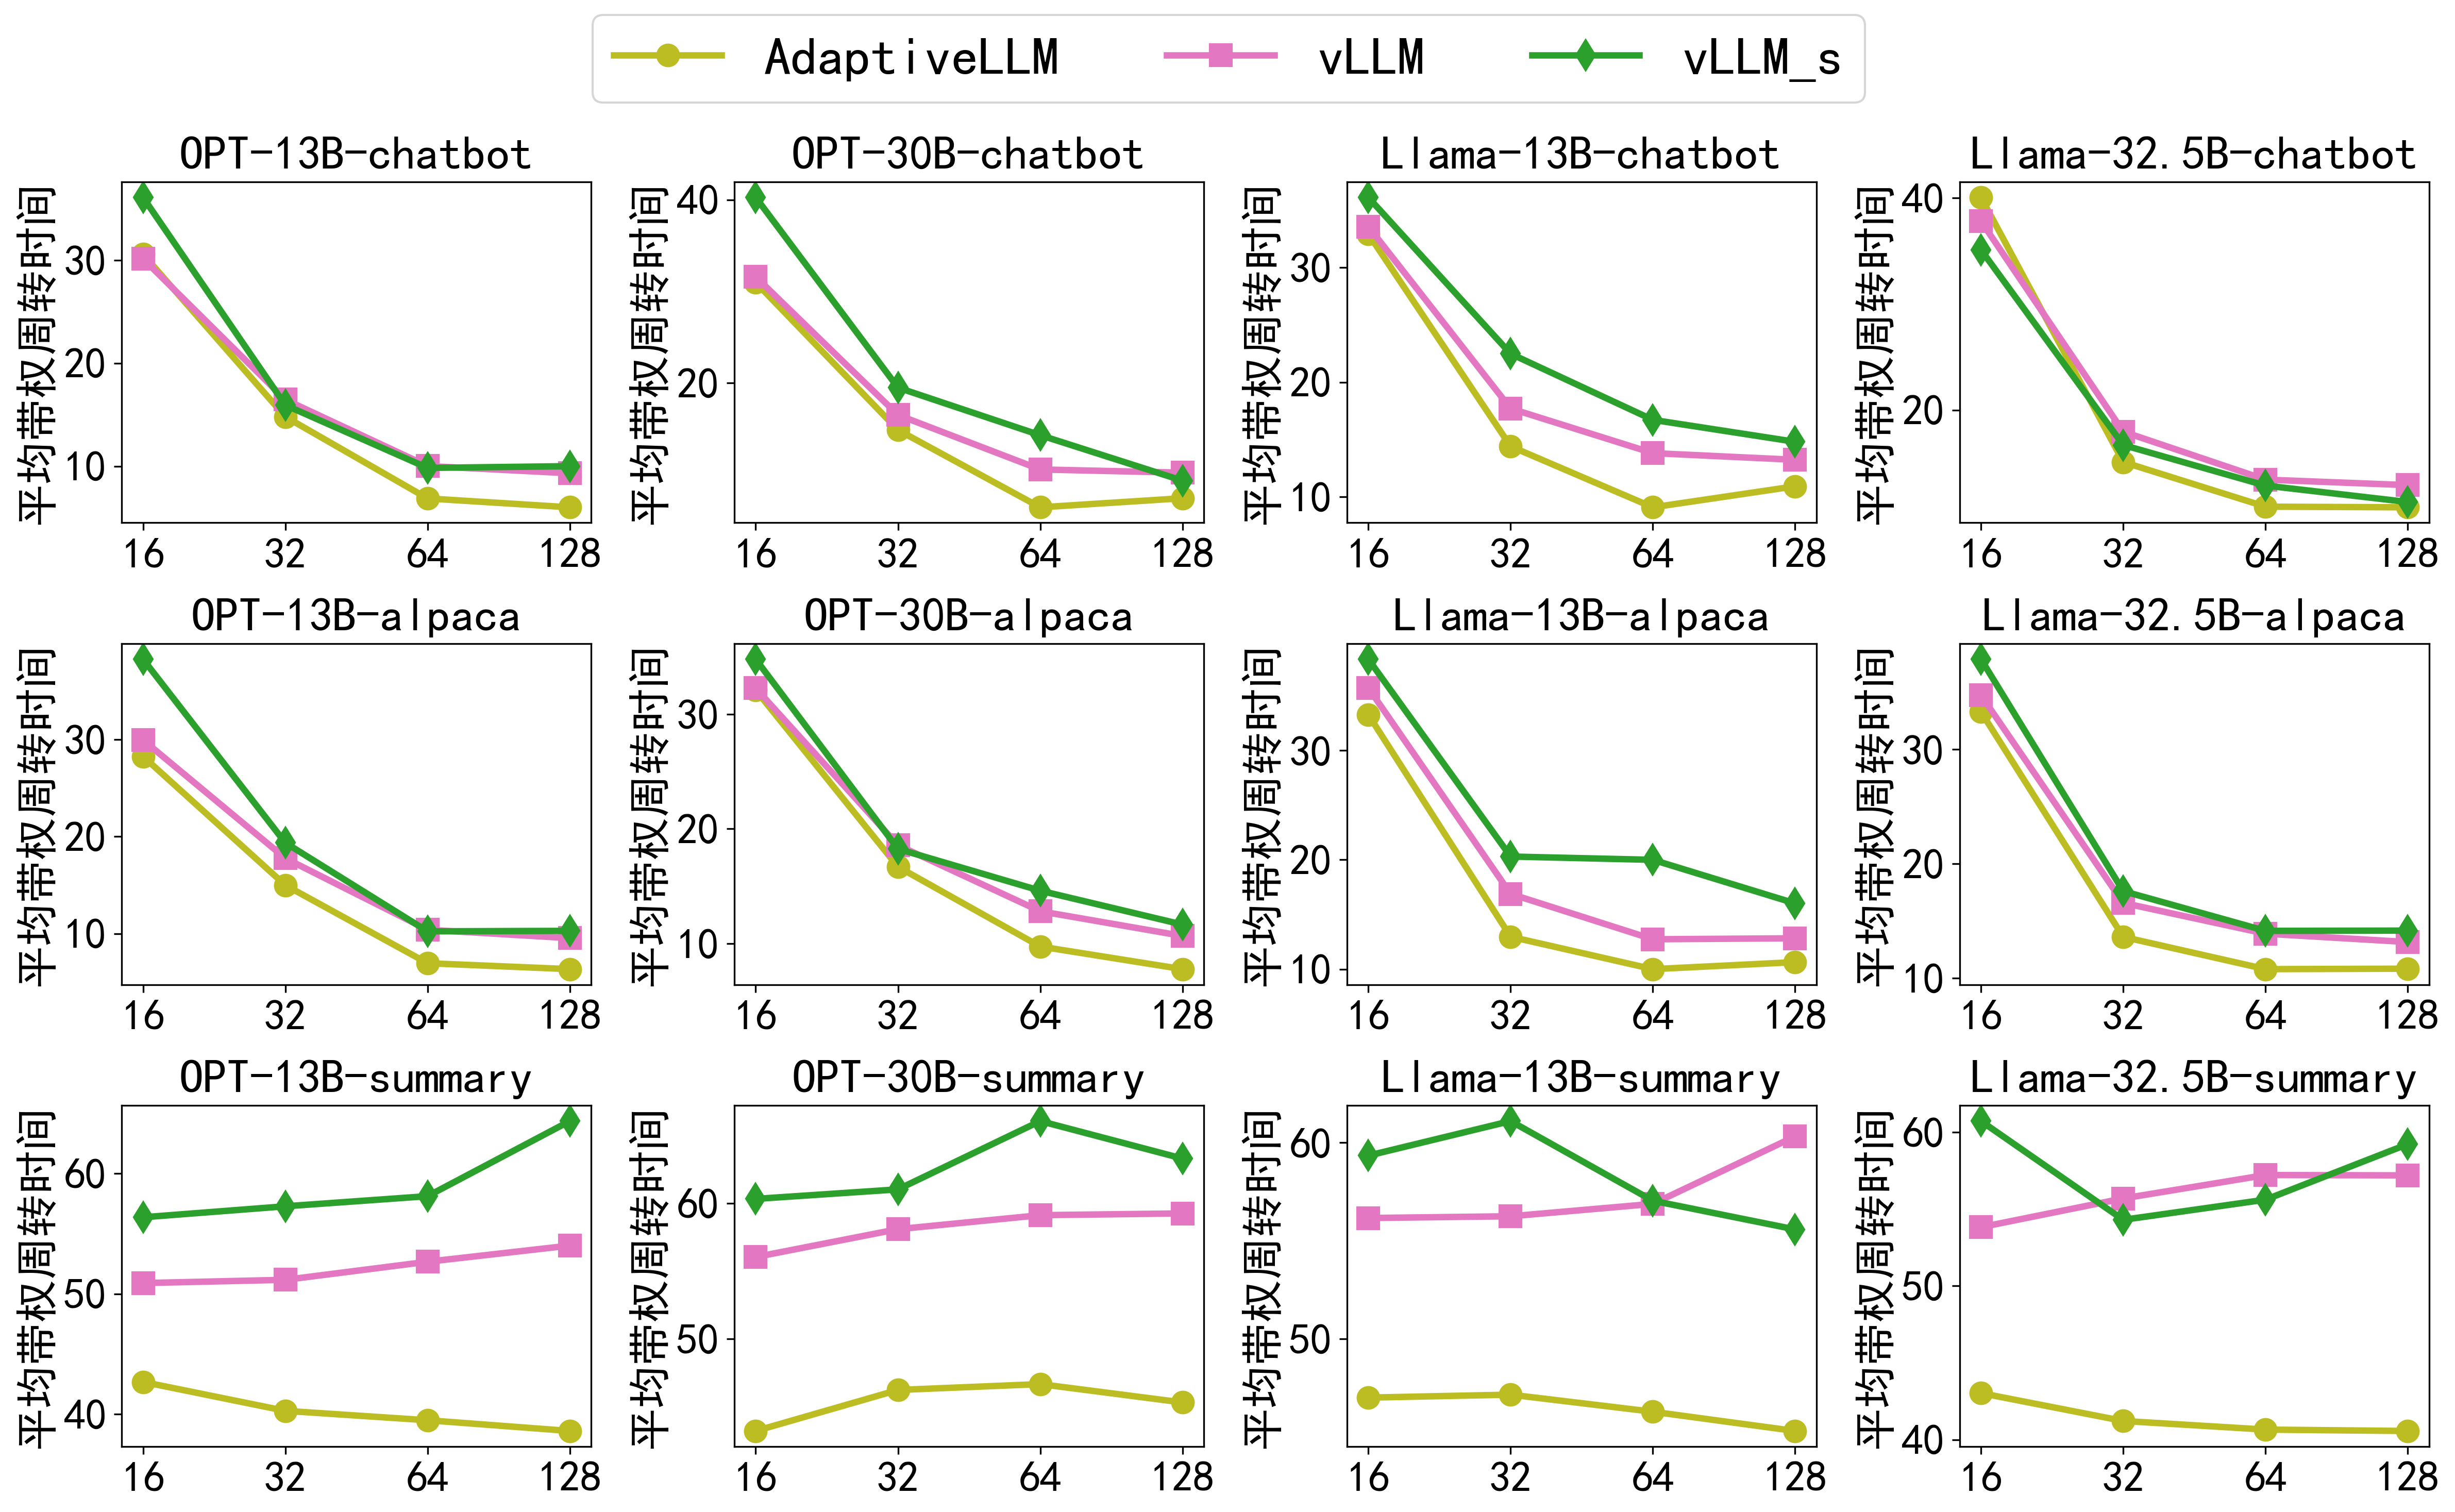
\includegraphics[width=0.9\linewidth]{用户请求平均带权周转时间.png}
  \caption{用户请求平均带权周转时间}
  \label{Fig:平均带权周转时间}
\end{figure*}

\subsection{实时性测试}

%wsq 公式中需要说明各个变量都是什么
为了消除整体吞吐率变化对实时性测试的影响,本文选取平均带权周转时间作为测试指标。用户请求带权周转时间等于客户端响应时间除以服务器端处理时间,如公式\ref{Eq:Weighted Around Time}所示。对于某一用户请求来说,$finish\_t$是其处理完毕时刻,$send\_t$是其从客户端发送至服务器端的时刻,$sche\_t$是其被AdaptiveLLM初次调度的时刻。平均带权周转时间($\geq 1$)越低,说明用户请求处理过程中的排队时间占比越低。 

\begin{equation}
  \begin{aligned}
    w\_around\_t = \frac{finish\_t - send\_t}{finish\_t - sche\_t}
  \end{aligned}
  \label{Eq:Weighted Around Time}
  \setlength{\abovedisplayskip}{0ex}
  \setlength{\belowdisplayskip}{2ex}
\end{equation}

%wsq 阐述一下和vllm_s的比较结果。此外图片中vllm's改成vllm_s

图\ref{Fig:平均带权周转时间}展示了平均带权周转时间随批处理大小上限的变化情况。在不同批处理大小设置下,基于公平性的用户请求调度策略均能使平均带权周转时间显著下降。当批处理大小较大时(64或128),AdaptiveLLM的平均带权周转时间相比于vLLM下降了20\%至40\%,相比于vLLM$\_$s下降了20\%至60\%。

对于序列较短的Chatbot和Alpaca数据集而言,随着批处理大小的上升,GPU利用更加充分,因此平均带权周转时间下降。在实际运行中,当批处理大小到达64至128时,GPU产生内存瓶颈,此时批处理大小无法继续提升,平均带权周转时间达到最小值。

对于序列较长的Summary数据集而言,其处理并发度被限制在较低水平(10以下),无法达到用户设置的批处理大小上限。因此平均带权周转时间呈稳定状态。AdaptiveLLM中高效的调度策略展现优势,使用户请求等待时间显著低于vLLM和vLLM\_s。

综上所述,基于公平性的用户请求调度策略使得用户请求从客户端发送至服务器端后能够很快开始处理,不会出现长时间等待现象。

\subsection{预测误差测试}

\subsubsection{张量重算预测误差}

张量重算开销由张量重算开销分析器根据LLM层数、LLM隐藏维度、单请求需要处理的token数量、以及批处理大小预测得到。表\ref{Table:OPT模型单步迭代执行时间预测误差}和表\ref{Table:LLama模型单步迭代执行时间预测误差}分别展示了OPT模型和Llama模型单步推理执行时间的预测效果。OPT执行时间预测任务共有6.4w条训练数据和1.6w条测试数据,结果表明,随机森林回归模型性能最佳,其在拟合2次多项式时能够达到1.76\%的预测误差。Llama执行时间预测任务共有6.8条训练数据和1.7w条测试数据,结果表明,随机森林模型同样性能最佳,其在拟合2次多项式时能够达到1.30\%的预测误差。

\begin{table}[H]
  \centering
  \caption{OPT模型单步迭代执行时间预测误差}
  \label{Table:OPT模型单步迭代执行时间预测误差}
  \renewcommand{\arraystretch}{1.25}
  \small
  \begin{tabular}{c c c c c c}
    \toprule
    \textbf{模型-拟合次数} & \textbf{1} & \textbf{2} & \textbf{3} & \textbf{4} & \textbf{5} \\
    \midrule
    线性回归模型 & 46.52 & 46.65 & 28.75 & 11.86 & 9.32 \\ 
    决策树 & 1.81 & 1.81 & 1.81 & 1.81 & 1.81 \\ 
    随机森林 & 1.77 & 1.76 & 1.77 & 1.77 & 1.78 \\ 
    岭回归模型 & 46.52 & 46.37 & 28.45 & 11.51 & 7.36 \\ 
    lasso回归模型 & 40.22 & 25.53 & 27.38 & 26.08 & 25.49 \\ 
    弹性回归模型 & 111.89 & 123.62 & 91.67 & 87.59 & 86.48 \\ 
    梯度提升模型 & 15.57 & 16.05 & 14.80 & 15.09 & 14.68 \\ 
    KNN回归模型 & 2.55 & 2.80 & 2.89 & 3.00 & 3.05 \\ 
    \bottomrule
  \end{tabular}
\end{table}

\begin{table}[H]
  \centering
  \caption{LLama模型单步迭代执行时间预测误差}
  \label{Table:LLama模型单步迭代执行时间预测误差}
  \renewcommand{\arraystretch}{1.25}
  \small
  \begin{tabular}{c c c c c c}
    \toprule
    \textbf{模型-拟合次数} & \textbf{1} & \textbf{2} & \textbf{3} & \textbf{4} & \textbf{5} \\
    \midrule
    线性回归模型 & 76.41 & 69.44 & 39.61 & 12.91 & 9.18 \\ 
    决策树 & 1.33 & 1.32 & 1.33 & 1.33 & 1.34 \\ 
    随机森林 & 1.31 & 1.30 & 1.31 & 1.31 & 1.31 \\ 
    岭回归模型 & 76.41 & 69.01 & 39.18 & 12.73 & 7.72 \\ 
    lasso回归模型 & 69.23 & 33.57 & 34.42 & 35.16 & 31.58  \\ 
    弹性回归模型 & 127.18 & 139.7 & 100.18 & 94.94 & 93.51  \\ 
    梯度提升模型 & 22.42 & 21.97 & 19.42 & 19.99 & 19.38  \\ 
    KNN回归模型 & 2.24 & 2.36 & 2.48 & 2.63 & 2.68 \\ 
    \bottomrule
  \end{tabular}
\end{table}

% \subsection{其它测试}

% wsq 合并到前面
\subsubsection{张量交换预测误差}

张量交换预测开销由张量交换开销分析器根据用户请求的KV Cache内存占用和GPU-CPU双向传输带宽而计算得到。本文针对模型Llama-13B和Llama-32.5B进行测试,其结果如图\ref{Fig:交换开销预测误差}所示。两个模型换入开销预测的MAPE误差分别为1.5\%和1.1\%,换出开销预测的MAPE误差分别为1.0\%和1.2\%。因此,张量交换开销总预测误差低于4\%。

\begin{figure}[!htbp]
  \centering
  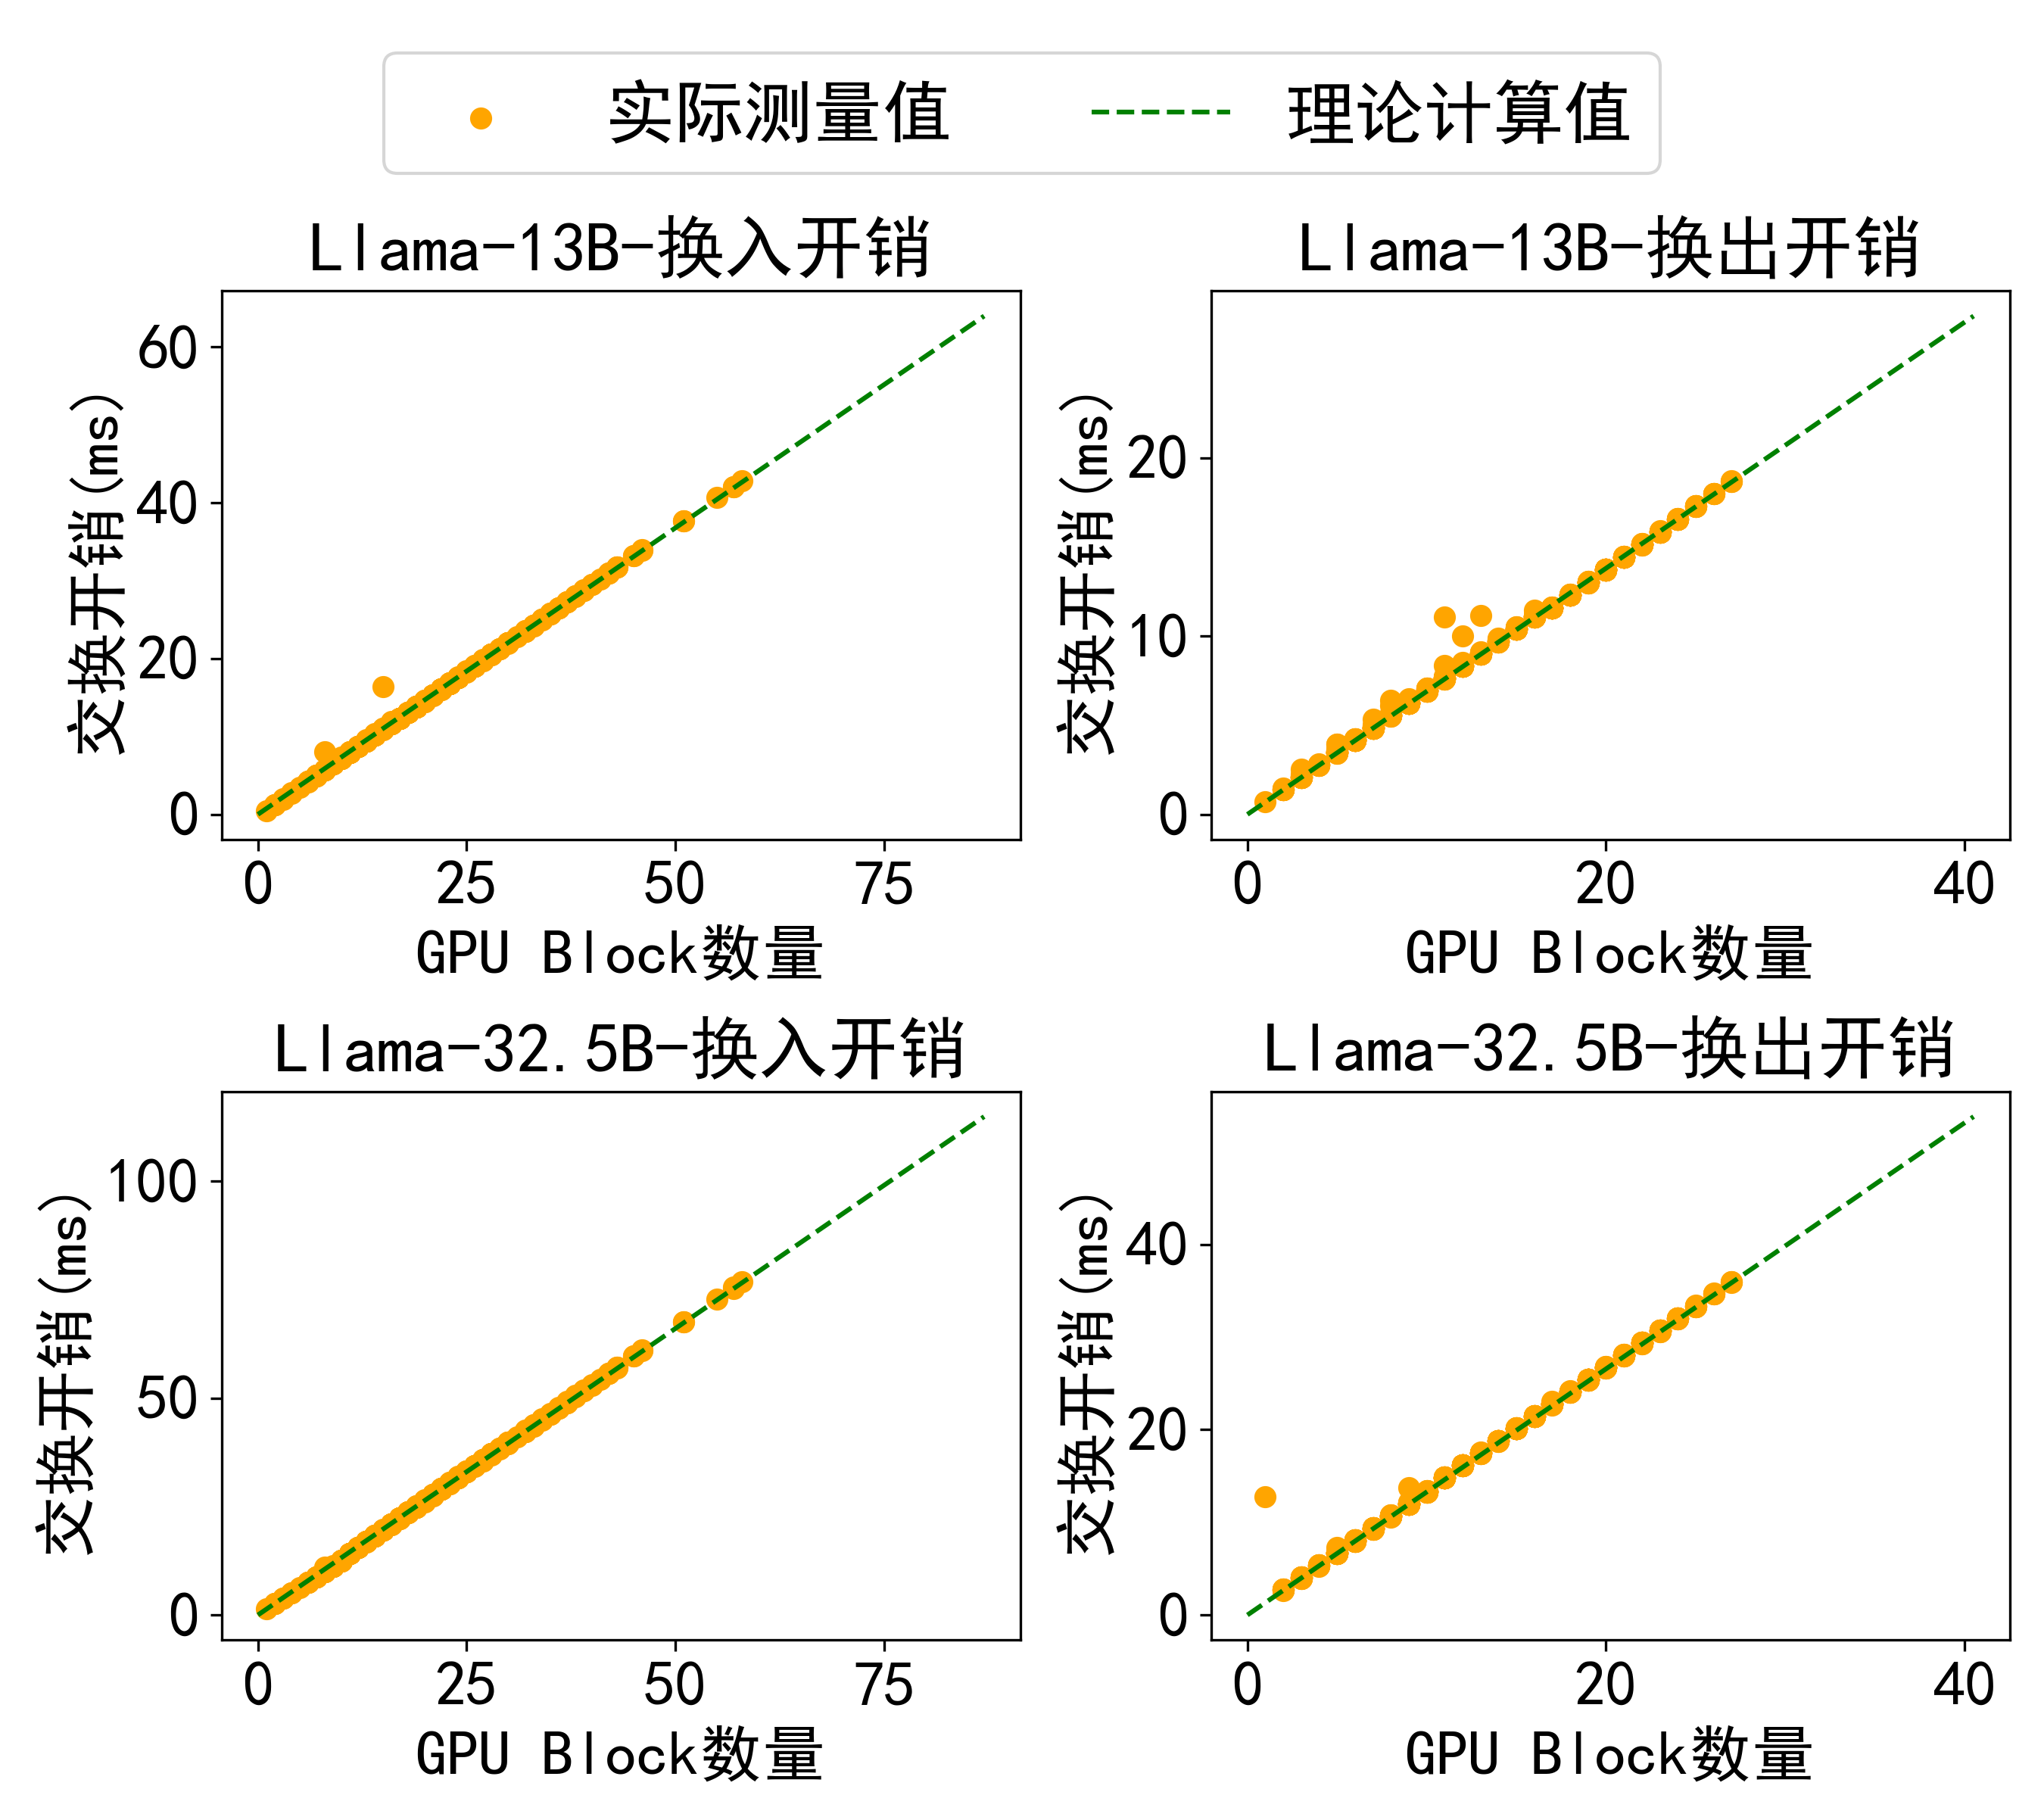
\includegraphics[width=0.9\linewidth]{交换开销预测误差.png}
  \caption{交换开销预测误差}
  \label{Fig:交换开销预测误差}
\end{figure}

\subsection{开销测试}

基于开销感知的内存优化策略在获取张量重算和张量交换开销时,会带来新的预测开销。本文设计如下对照实验获取预测过程的开销:在吞吐率测试过程中,当GPU内存不足时调用开销比较过程,但最终使用vLLM提供的固定式内存优化策略(张量重算)。观察此情景下推理任务的总用时可知,预测开销在推理任务中仅占0.1\%至1\%。

基于公平性的用户请求调度策略也有一定的开销。理论上,该算法的时间复杂度为$O(r^2)$,其中$r$为running队列中用户请求的数量。在实际运行过程中,每次调度的开销在0.2ms左右,总开销在推理任务中仅占0.5\%至1\%。综上所述,AdaptiveLLM引入的两种优化策略所带来的额外开销均可忽略不计。
